\documentclass{article}

\usepackage{fancyhdr}
\usepackage{ragged2e}
\usepackage{graphicx}
\usepackage{caption}
\usepackage{geometry}
\usepackage{amsmath}
\usepackage{rotating}

\usepackage{listings}
\usepackage{color}

\definecolor{dkgreen}{rgb}{0,0.6,0}
\definecolor{gray}{rgb}{0.5,0.5,0.5}
\definecolor{mauve}{rgb}{0.58,0,0.82}

\lstset{frame=tb,
  language=Java,
  aboveskip=3mm,
  belowskip=3mm,
  showstringspaces=false,
  columns=flexible,
  basicstyle={\small\ttfamily},
  numbers=none,
  numberstyle=\tiny\color{gray},
  keywordstyle=\color{blue},
  commentstyle=\color{dkgreen},
  stringstyle=\color{mauve},
  breaklines=true,
  breakatwhitespace=true,
  tabsize=4
}

\setcounter{secnumdepth}{1}

\usepackage{chngcntr}
\counterwithin{figure}{section}

\renewcommand*{\thepage}{C\arabic{page}}

\pagestyle{fancy}
\lhead{ACME Robotics}
\chead{\#8367}
\rhead{\ifcontents Contents \else Week \thesection \fi}

\newif\ifcontents
\contentstrue

\makeatletter
\renewcommand{\@seccntformat}[1]{}
\makeatother

\begin{document}\contentsfalse
\subsection{Sorter CAD}
%! CAD the sorter.
Ashlin and Aidan continued to finalize the sorting system for the robot and completed the CAD model of the sorter. Aidan realized a flaw with the system, if a ball then a cube went into the sorter right after each other then the cube could jam the sorter. This was because the interior length of the rotating piece was almost 4 inches long, so if a ball then a cube went in the sensor would read the ball and then start rotate but the cube would block the rotating and jam the servo. Kelly, Ashlin, Aidan, and Jon all thought of ideas to solve this problem including shortening the sorter's dimensions, creating a servo powered gate, or just changing the whole system. The team finally decided to solve the problem once the sorter was fabricated. The problem could only occur if the two items went into the sorter immediately after each other. The team believed that the intake would probably space out the items sufficiently so this problem wouldn't occur, and if it did occur small adjustments could be made to increase the space between items.

\subsection{Develop custom lift}
%! Further investigate possible lift designs and weigh the pros and cons of each. 
The x-rail lift design would work, but Kelly still wanted to investigate another type of lift, with square tubing, bearings, and custom bearing blocks. While more labor-intensive and harder to pull off, the end result would be better than with x-rail if it turned out correctly. Where the x-rail only needed bearings on one side, because the v-bearings would be able to resolve both radial and lateral loads, normal bearings can only resolve radial loads, so bearings will have to be placed on at least three sides to constrain the lift in both dimensions. Since the lift is composed of two mirrored parts, connected by the frame of the first stage, Kelly could get away with only running bearings along three sides of each tube, excluding the outer one, because the bearings in the y-axis would push the two sides against each other, preventing the lift from shifting side-to-side. Each bearing assembly would consist of four bearings, two on either side of the tube pinching it, and two next to each other running along the inside of the tube. Kelly began the CAD by making 1 in by $\frac{1}{2}$ in by $\frac{1}{16}$ in wall aluminum tubing in 16 inch lengths. One of these would be mounted to the drivetrain, and the other would make up the vertical portion of the first stage, rolling along the fixed one. A bearing assembly would go at the top of the fixed one and the bottom of the moving one, keeping the bearings as far apart from each other as possible, distributing the load and stabilizing the lift. The inner carriage would be made out of a H-shaped arrangement of more tubes, with a bearing assembly mounted at the top and bottom of each side of the H. After considering mounting the bearings by sandwiching the tube between two machined plates, Kelly realized this would not support the inner bearings, so decided on machined blocks that would be fixed to the tube with rivets. The blocks would have a quarter inch hole on the side for attaching the pinching bearings, and hole at the top where a bolt would connect the two blocks and support the inner bearings. After assembling this, Kelly found there was not enough room on the vertical portion of the first stage for both sets of bearings to roll against it, so it was necessary for them to be swapped out for one inch by one inch tubes instead. 

\subsection{CAD Lander Clamp}
%! Create a latch in CAD that will be used to attach to the lander. 
To lower and raise the robot from the lander, the team decided to attach a latch to their lift. The team decided to do this because by attaching it to the scoring lift the team would not have to create a separate lift or arm to hang from. Kelly made the original prototype for this mechanism - which used two pillow blocks that when placed around the hook on the lander had a bar slid through to have the robot hang. Jon then used this basic prototype to CAD a more finalized design.

\begin{figure}
    \centering
    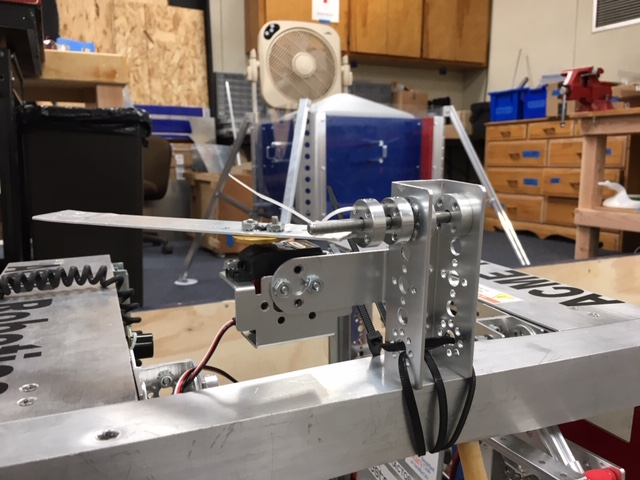
\includegraphics[width=.6 \textwidth]{06_10-08/images/latch1.JPG}
    \caption{Latch Prototype}
    \label{fig: Latch CAD1}
\end{figure}

\begin{figure}
    \centering
    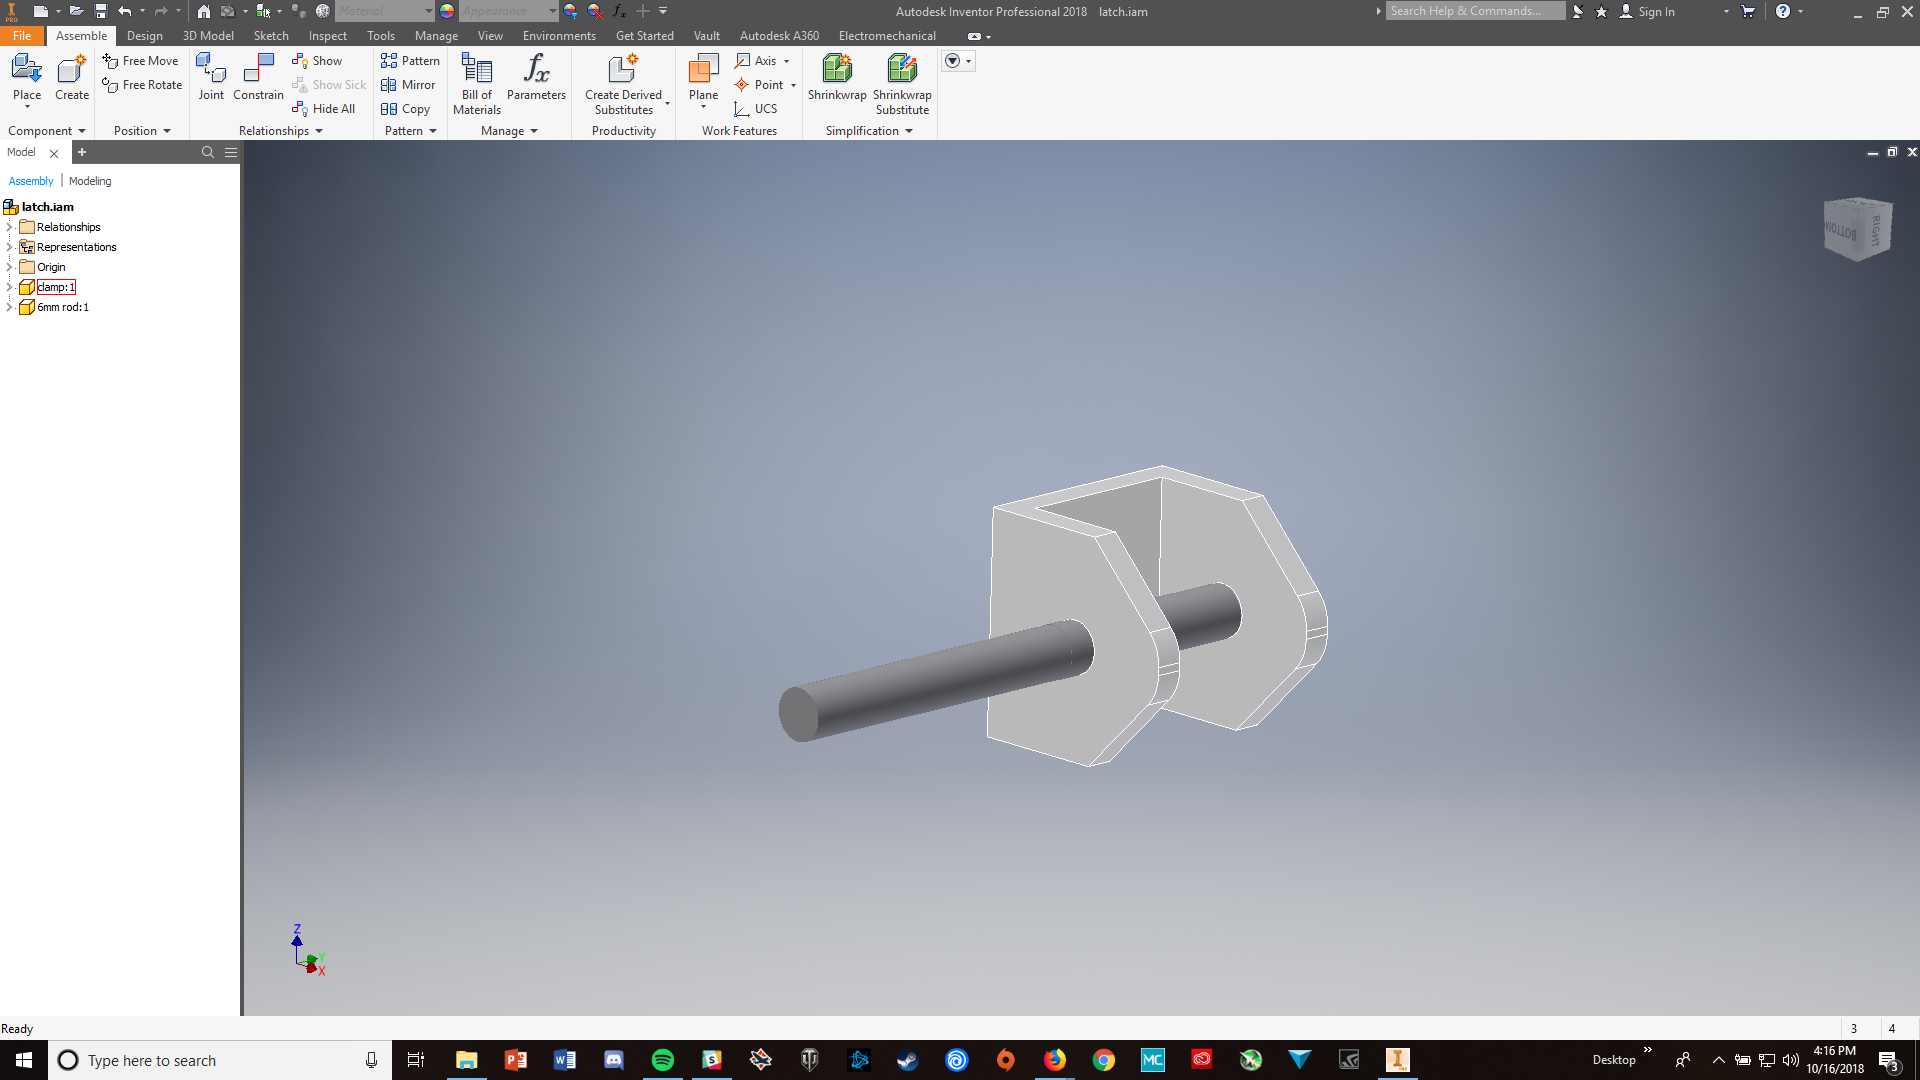
\includegraphics[width=.6 \textwidth]{06_10-08/images/latch.png}
    \caption{Latch CAD}
    \label{fig: Latch CAD2}
\end{figure}

\subsection{Finalize robot design}
%! Discuss the final robot design with the team.
The team got together and went over the robot design, making sure that everything had been considered and accounted for before the final stages of CAD were completed and parts were ordered. Everybody presented prototypes and CAD that they had been working on, and the team decided whether or not to stick with it, and discussed any problems that might arise as the parts went into production. The first thing to decide was the type of drive base. The team had used mecanum drives the previous two years, and was confident they could build it correctly, but did not want to dismiss a tank drive. The tank drive that was being considered was a chain driven 6-wheel drop center west coast drive. The mecanum drive being considered was the same thing that the team had used to success last year, a belt-driven mecanum drive, with dead axles constrained between drive plates giving it extra rigidity. Oren had made some improvements over last year's design, including using smaller belts and swapping out parts to increase maintainability. The team decided they should use mecanum drive for its increased maneuverability unless a definite need for tank drive was needed. Because the defensive advantage given by the advantage of tank was countered by the maneuverability of mecanum and the ability to get out of tight situations, and the settled upon intake had no need for the robot to be able to go inside the crater, the team decided to go with a mecanum drive. The team decided to stick with the intake design consisting of a rake that would extend over the crater wall and pull minerals toward the robot and a series of surgical-tubing whips to suck the minerals in from there. The active sorter using a color sensor was chosen because it would be more reliable when the robot was in motion, and the double cartridge design was chosen because it would allow the two mineral types to be scored independently. Finally, the team decided to use the custom lift rather than the x-rail based one because Oren was confident that he would have the time to manufacture it to the neccecary specifications, and Dan felt it was something that would be able to be made on the manual mill at GSS.

\begin{figure}
    \centering
    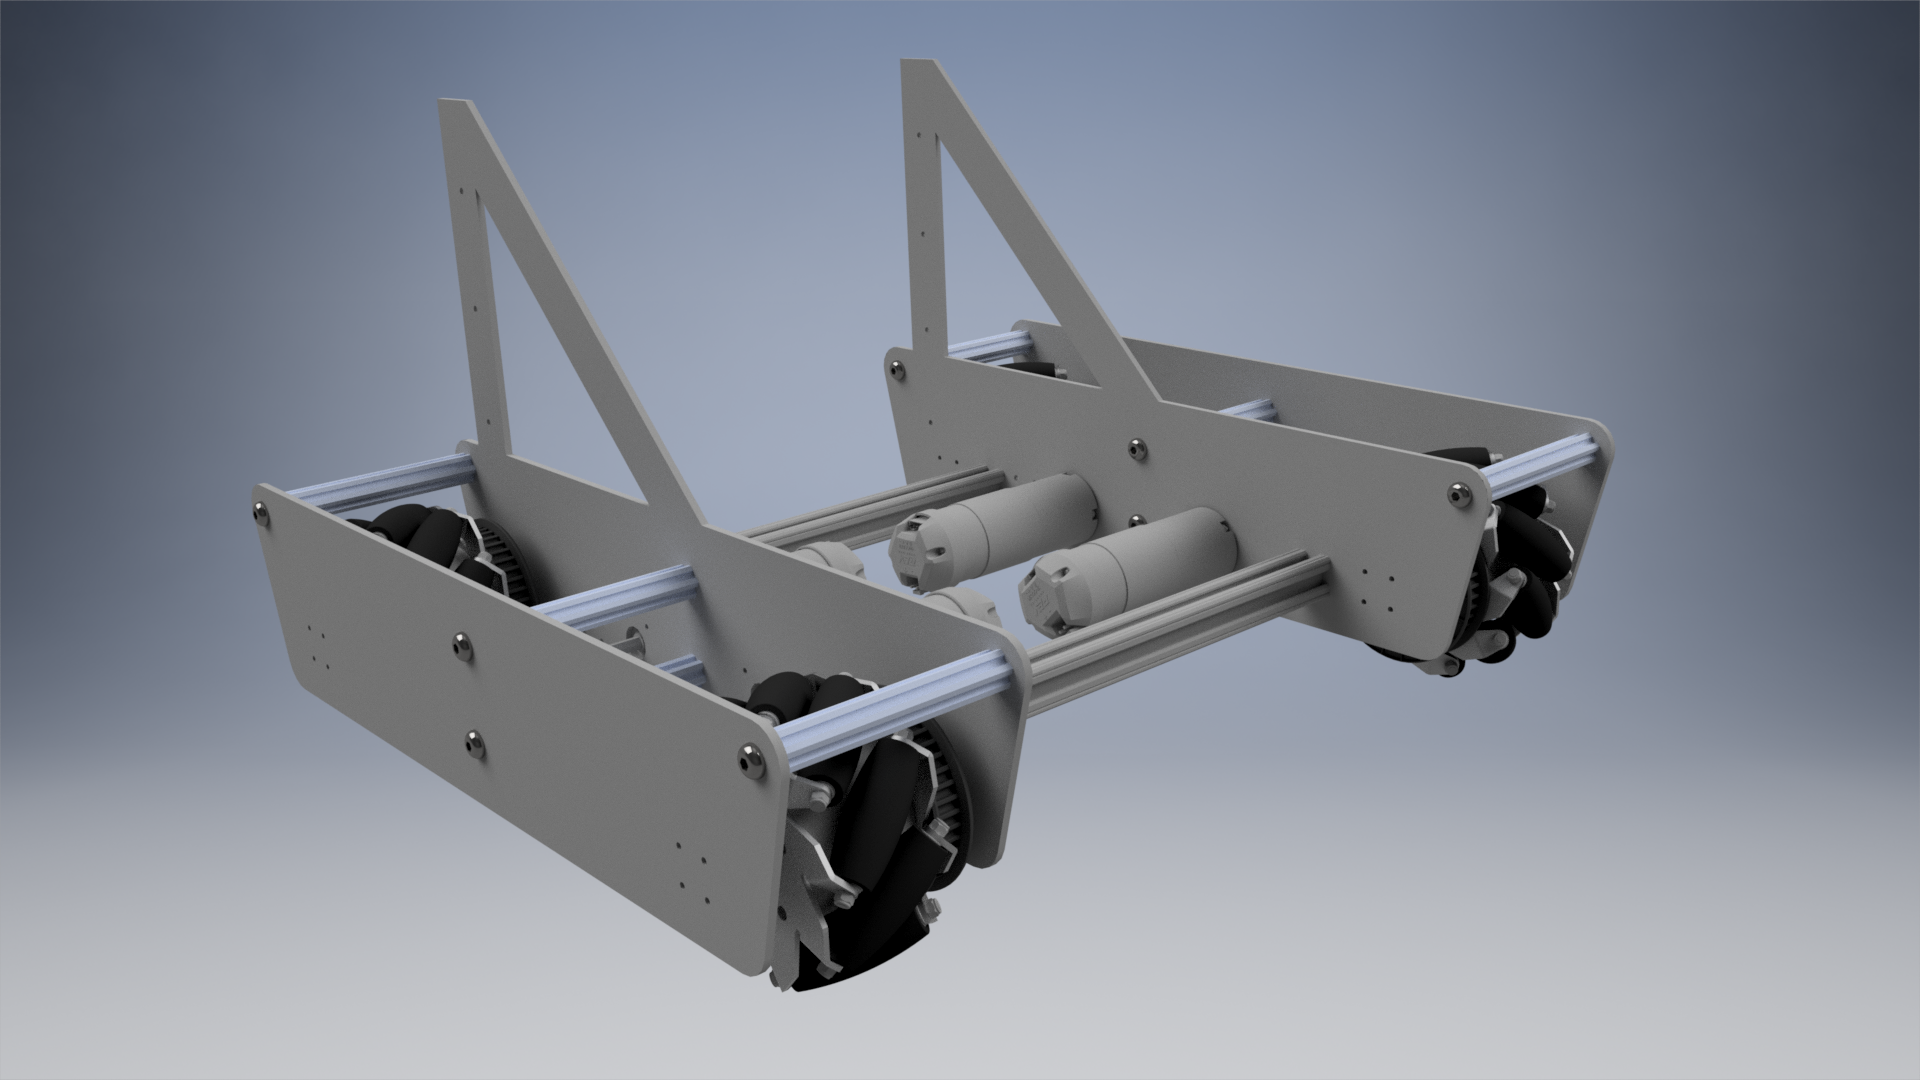
\includegraphics[width=.6 \textwidth, ]{06_10-08/images/robot[1].png}
    \caption{Drive train CAD}
    \label{Dive train CAD}
\end{figure}
\end{document}

